\documentclass[12pt,a4paper]{report} 
\usepackage[utf8]{inputenc}
\usepackage[russian]{babel}
\usepackage[T2A]{fontenc}
\usepackage{amsmath}
\usepackage{amsfonts}
\usepackage{amssymb}
\usepackage{hyperref}
\ifx\pdfoutput\undefined
\usepackage{graphicx}
\else
\usepackage[pdftex]{graphicx}
\fi
\graphicspath{{images/}{lab/img_lab_3/}}
\usepackage{longtable}
\usepackage[left=2cm,right=2cm,top=2cm,bottom=2cm]{geometry}
%
\newtheorem{Task}{Задача}
\newtheorem{Example}{Пример}
%Параметры титульного листа
\author{Цымай Д.В.\\ \texttt{dmitryzy@gmail.com}}
\title{Практические занятия \\ по курсу "Физическая и коллоидная химия"}
\date{}
%
\begin{document}
\section{Лабораторная работа 3 }
\textbf{Тема:}Построение диаграмм состояния трехкомпонентной системы с ограниченной взаимной растворимостью.

\textbf{Цель работы:}Построить диаграмму состояния тройной системы $CH_{3}COOH$ --- $CH_{3}Cl$ --- $H_{2}O$.

\textbf{Оборудование и реактивы:} бюретка, 8 колб, с притёртыми пробками на 200 мл, пипетка на 5 мл, мерный цилиндр на 50 мл, раствор $CH_{3}COOH$, раствор $CH_{3}Cl$.

\textbf{Теория}

Физико-химический анализ  устанавливает  количественную зависимость между составом и каким-нибудь измеренным физическим свойством  системы (температурой кипения,  плавления,  давления пара, электропроводностью и др.) Графическое изображение зависимости какого либо свойства от состава системы или другого фактора равновесии ее (например, давления) называется диаграммой состояния. Диаграммы состояния позволяют сделать выводы о взаимодействиях отдельных веществ в системе,  образования новых  химических  соединений, твердых растворов, их составе и границе существования.

Для разбора диаграмм состояния широко применяется теория равновесия  неоднородных (гетерогенных) систем,  прежде всего -- правило фаз Гиббса.

Ознакомившись с сущностью физико-химического анализа,  его значением,  с понятием фаза,  компонент и степени свободы,  обратите внимание на следующее: фаза не адекватна понятию агрегатного состояния и в однокомпонентных системах в равновесии могут находиться две фазы одного агрегатного состояния.

Число степеней свободы ($C$) определяется числом компонентов ($K$) и фаз ($F$), находящихся  в  равновесной  системе ($C=K+2-F$).

Студентам необходимо  приобрести  навыки  чтения  диаграмм состав-свойство различных бинарных жидких смесей,  диаграмм плавкости и простейших диаграмм трехкомпонентных систем. При выполнении лабораторной работы необходимо научиться определять в любой точке на диаграмме число компонентов и фаз,  состав системы и весовые соотношения компонентов,  уметь находить температуру  начала  и  конца кристаллизации и плавления,  кипения и конденсации. Надо знать, на основании каких экспериментальных данных строятся различные  диаграммы.

В тех случаях, когда система состоит из трех компонентов, пользуются треугольником Гиббса. Принимают, что каждая вершина равностороннего треугольника отвечает 100\% составу одного из  компонентов,  а каждая сторона -- двойной системе из компонентов, указанных в вершинах, которые она соединяет.

\begin{figure}[h]
\center{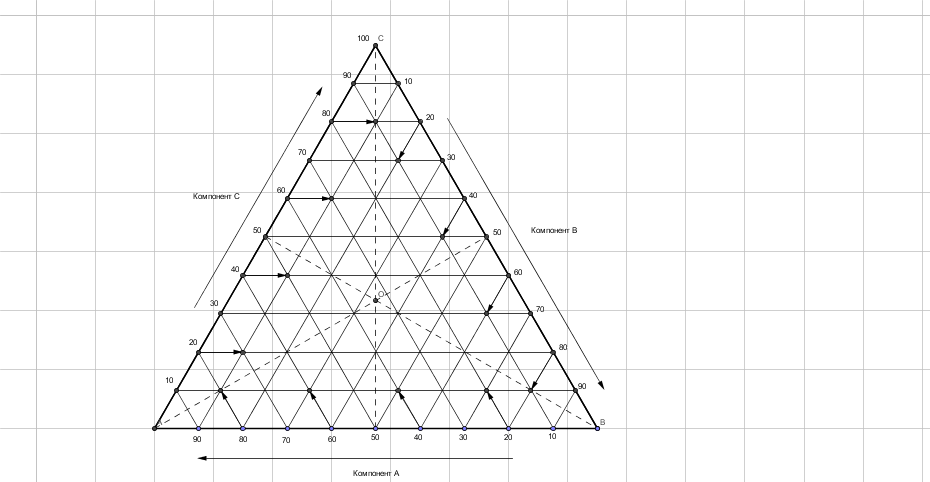
\includegraphics[width=0.5\linewidth]{gibbs.png}}
\caption{Треугольник Гиббса}
\label{ris:image}
\end{figure}

В треугольнике проводят три высоты,  делят каждую высоту на десять равных отрезков и через полученные деления проводят прямые, с помощью которых можно представить любой состав тройной системы.

Чтобы нанести точку, отвечающую составу трехкомпонентной системы, на двух высотах откладывают процентное содержание соот-ветствующих компонентов.  Через полученные точки на высотах проводят прямые,  параллельные сторонам, лежащим против угла, вершина которого отвечает содержанию чистого компонента.  Точка пересечения  прямых будет отвечать искомому составу.

\textbf{Порядок выполнения}

1. В 8  Колб  с  притертыми  пробками наливают по 10 мл бинарных смесей взаимно растворимых друг в друге веществ ($CH_{3}COOH$ --- $CH_{3}Cl$)  в соотношении, указанном в таблице \ref{tabular:data3}.

\begin{table}[h]
\caption{Объемы компонентов бинарных смесей}
\label{tabular:data3}
\begin{center}
\begin{tabular}{|p{6cm}|c|c|c|c|c|c|c|c|}
\hline
\No колбы & 1 & 2 & 3 & 4 & 5 & 6 & 7 & 8 \\
\hline
Объем $CH_{3}COOH$, мл & 2 & 4 & 6 & 7 & 7,5 & 8 & 8,5 & 9 \\
\hline
Объем $CH_{3}Cl$, мл & 8 & 6 & 4 & 3 & 2,5 & 2 & 1,5 & 1 \\
\hline
Объем $H_{2}O$, мл & & & & & & & &  \\
\hline
\end{tabular}
\end{center}
\end{table}

2. Растворы титруют водой до появления мути.  В некоторых опытах для этого достаточно одной-двух капель воды.  Результаты занося  в таблицу \ref{tabular:data3}.

\textbf{Обработка экспериментальных данных}

1. Для расчёта количеств веществ компонентов пользуются формулой:
$$n=\frac{V \cdot \rho}{M}$$
где $n$ - количество вещества, моль;

$V$ - объем вещества, мл;

$\rho$ - плотность (приведена в таблице \ref{tabular:data4});

$M$ - Молярная масса, г/моль.

Рассчитайте молярные массы компонентов и занесите результат в таблицу \ref{tabular:data4}.

\begin{table}[h]
\caption{Данные для рассчета}
\label{tabular:data4}
\begin{center}
\begin{tabular}{|p{5cm}|p{5cm}|p{5cm}|}
\hline
Вещество & Плотность, г/мл & Молярная масса, г/моль\\
\hline
$CH_{3}COOH$ & 1,06 & \\
\hline
$CH_{3}Cl$ & 1,5 &  \\
\hline
$H_{2}O$ & 1,0 &  \\
\hline
\end{tabular}
\end{center}
\end{table}

2. Рассчитать количество вещества компонентов системы, результат занести в таблицу \ref{tabular:data5}.

\begin{table}[h]
\caption{Состав бинарных смесей, моль}
\label{tabular:data5}
\begin{center}
\begin{tabular}{|p{8cm}|c|c|c|c|c|c|c|c|}
\hline
\No колбы & 1 & 2 & 3 & 4 & 5 & 6 & 7 & 8 \\
\hline
Количество вещества $CH_{3}COOH$, моль & & & & & & & & \\
\hline
Количество вещества $CH_{3}Cl$, моль & & & & & & & & \\
\hline
Количество вещества $H_{2}O$, моль & & & & & & & &  \\
\hline
Всего, моль & & & & & & & &  \\
\hline
\end{tabular}
\end{center}
\end{table}

3. Рассчитывают состав системы в мольных долях, отвечающий началу расслоения (появления мути).
Мольной долей компонента ($x$) считают  отношение  числа молей данного компонента к сумме молей всех компонентов раствора. Например, мольную долю компонента $A$ вычисляют по уравнению:
$$x=\frac{n_{A}}{n_{A}+n_{B}+n_{C}}$$
Мольные доли других компонентов вычисляют по подобным уравнениям. Результаты рассчетов занести в таблицу \ref{tabular:data5}. Сумма мольных долей всех компонентов должна быть равна $1$.

4. Полученные данные наносят на треугольную диаграмму.  Соединив точки, получают плавную кривую,  по одну сторону которой находится гетерогенная область, по другую -- гомогенная.

\begin{table}[h]
\caption{Состав бинарных смесей, мольные \%}
\label{tabular:data3}
\begin{center}
\begin{tabular}{|p{8cm}|c|c|c|c|c|c|c|c|}
\hline
\No колбы & 1 & 2 & 3 & 4 & 5 & 6 & 7 & 8 \\
\hline
Мольная доля $CH_{3}COOH$, \% & & & & & & & & \\
\hline
Мольная доля $CH_{3}Cl$, \% & & & & & & & & \\
\hline
Мольная доля $H_{2}O$, \% & & & & & & & &  \\
\hline
Всего & & & & & & & &  \\
\hline
\end{tabular}
\end{center}
\end{table}

\textbf{Контрольные вопросы}
\begin{enumerate}
\item Что называется фазой, компонентом и степенью свободы? 
\item В чем заключается физико-химический метод анализа? 
\item На чем основан термический анализ ?
\item Как изображается состав трехкомпонентной системы по методу Гиббса?
\item В чем заключается процесс экстрагирования,  какова его теоретическая основа?
\item Что такое мольная доля?
\item Что такое химический потенциал?
\item Закон распределения.
\item Правило фаз Гиббса.
\end{enumerate}
\end{document}